\documentclass[twocolumn,10pt]{article}
\usepackage[T1]{fontenc}
\usepackage[utf8]{inputenc}
\usepackage{amsmath}
%\usepackage[english]{babel}
%\usepackage{biblatex}
\usepackage[margin=.75in]{geometry}
\setlength{\columnsep}{33pt}
\setcounter{secnumdepth}{2}
\usepackage{minipage-marginpar}
\newcommand\vfilbreak[1]{\vskip 0pt plus #1 \penalty-200 \vskip 0pt plus -#1}
\newenvironment{mpmp}[1]
               {\begin{minipagewithmarginpars}{#1}}
               {\end{minipagewithmarginpars}}
\usepackage{morefloats}
\usepackage{booktabs}
\usepackage{color}
\usepackage{graphicx}

\title{Lung Cancer Detection Milestone}
\author{Jay DeStories, Jason Fan, Alex Tong}
\date{March 2017}

\newcommand{\red}[1]{{\color{red}#1}}
\newcommand{\temp}[1]{{\red{#1}\\}}
\renewcommand{\b}{\boldsymbol}

\usepackage{enumitem}

\begin{document}

\maketitle
\section{Introduction}

In this document, we record the intermediary results for the Multi-Instance
Network Lung Cancer Detection project.

Please refer to project proposal for references to the proposed pipeline and
techniques.

\subsection{Things we didn't expect to be so difficult}

Our team found the following two problems more difficult than expected:
\begin{enumerate}[noitemsep]
  \item Getting working implementation of AlexNet \cite{AlexNet} and learning TensorFlow
  \item Pre-processing Data and working with DICOM images
\end{enumerate}

\subsection{Problems with Preprocessing}

With the LUNA and Kaggle Dicom data amounts to almost a terabyte of storage, we
made some mistakes with data processing and had to process the Kaggle Data twice.

We had trouble converting Hounsville Units (hu), the unit of measurement for DICOM
slice densities, to a sensible numeric value a traditional image classification 
network would be able to consume. 

Hounsville Units measure density and map different parts of the human bodies to
a high range of values, we experimented with the DICOM slices to find appropriate
thresholded minimum and maximum values so that resulting images retained enough
contrast. You can see in Figure 2, that the lung scaled to reasonable pixel values
has very little contrast. In figure 4 you can see our rescaling and thresholding
efforts to improve the contrast of the image. We reason that the closer we can get
the histogram of the lung to look to a typical image in the ImageNet dataset, then
the better VGG will perform in discerning features on the lung image. 

We attempted to scale the image such that the lung had a black background and the majority
of the lung pixels were in the center range of pixel intensities. We speculate that it might
be advantageous to increase the contrast further (essentially stretch the bump in the middle
of Figure 3) so that our image histogram might look more like an ImageNet histogram.

\begin{figure}[h!]
  \label{fig:Uninterpreted Histogram}
  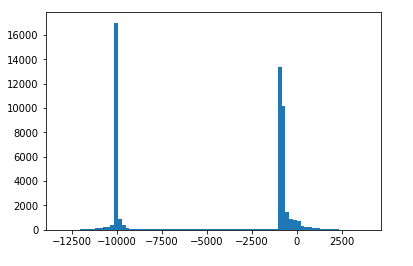
\includegraphics[width=\columnwidth]{img/hu_histogram.png}
  \caption{Histogram of Pixel Values of a resized interpolated lung}
\end{figure}
\begin{figure}[h!]
  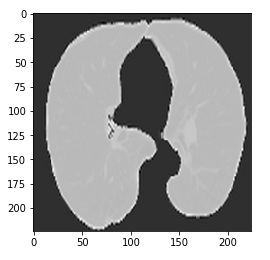
\includegraphics[width=\columnwidth]{img/slice_no_preprocessing.png}
  \caption{Lung Slice without preprocessing}
\end{figure}

\begin{figure}[h!]
  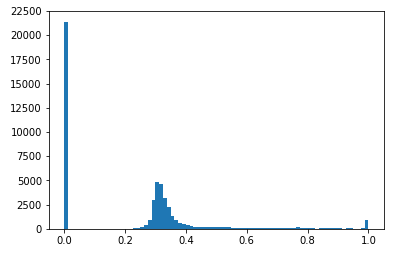
\includegraphics[width=\columnwidth]{img/scaled_histogram.png}
  \caption{Histogram of Pixel Values of a scaled resized interpolated lung}
\end{figure}

\begin{figure}[h!]
  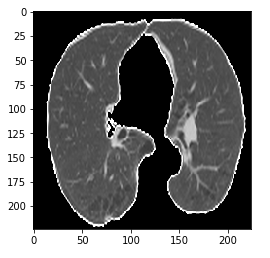
\includegraphics[width=\columnwidth]{img/threshold_image.png}
  \caption{Histogram of Pixel Values of a scaled thresholded resized interpolated lung}
\end{figure}

\subsection{From AlexNet in Keras to VGG in TensorFlow}

The Multi-Instance Network from the University of
California Irvine (UCI) researchers was implemented with a custom, unmaintained
version of Keras that we found, albeit too late, to be untenable. 

We decided to move to using TensorFlow for clearer documentation and more support
from the online community. At first, we found TensorFlow difficult to understand,
but we eventually found a simple enough implementation of VGG to work with.
(From: \texttt{github.com/machrisaa/tensorflow-vgg})

\section{Pipeline Progress}
We have implemented the following:
\begin{enumerate}[noitemsep]
  \item Memory concious RGB CNN to Grayscale CNN conversion
  \item Feature extraction with pre-trained VGG-16
  \item Feature extraction with pre-trained VGG-19
  \item Multi-Instance 2-class logistic regression
  \item Boosted decision tree
\end{enumerate}

\subsection{RGB to Grayscale conversion}
The Keras implementation of Multi-Instance Network feeds the first convolutional
an image of shape (224,224,3) in which the black and white dicom image is
copied once onto each Blue, Red and Green channel.

We attempted to mimic this technique with the stock VGG implementation to extract
slice-wise image features from the last fully convolutional layer and found that
we could not fit an entire lung volume into VRAM.

We noticed that for weight vector $\b w$ along the channels axis of a convolution, the
result of the convolution with pixel vector $\b x$ where each channel has value
$\hat x$, channelwise mean $\b \mu$ and bias
term $b$ was,

$$\b w \ast (\b x - \b \mu) + b = (\b w \ast \b x) + (b - \b w \ast \b \mu)
= \hat x \|\b w\|_1 + (b - \b w \ast \b \mu)$$

Which meant that we could eliminate the redundant 3-channel input dimension and
make any convolutional neural network effectively consume grayscale images by
 manipulating pretrained weights and biases for the first layer. We simply sum
 the convolution along the axis of the input channels dimension and subtract the
 term $(\b w \ast \b \mu)$ from the bias.

 We did this for both VGG-19 and VGG-19 and were able to forward pass entire
 lung volumes to extract slice-wise features.

\subsection{VGG feature extraction}

We perform the above mentioned RGB to Grayscale conversion for both VGG-16 and VGG-19 
and were able to reduce VRAM usage and forward pass entire lung volumes to 
extract slice-wise features \cite{simonyan2014vgg}. A feature tensor of shape (7, 7, 512) is extracted
for each slice, where each of the 49 receptive fields is represented by a feature
vector of length 512.

The resulting bag of features that is then consumed by the
Multi Instance 2-class Logistic Regression and Boosted Decision Tree Models,
is a tensor of shape (60, 7, 7, 512).

\subsection{Multi Instance 2-class logistic regression}
Let $F$ be a set of $N$ feature vectors that represent the instances of a given
lung slice. 
Then $\b r$, the vector of activations, is defined element wise by
$$r_i = \b w^T \b f_i + b$$.
Where $f_i$ and $r_i$ is the $i$-th element of $\b r$ and $F$ respectively.

We then use $\b r $ to predict the probability of cancer $p(y = 1)$ where
$$t = p(y = 1) = \max_{r_i} \ \sigma(r_i)$$

The authors of the Multi-Instance learning paper proposed the following per example loss functions
to regularize hyper-parameters at training time \cite{mil_mammogram}.

Normal softmax loss:
$$L_{max} = -\log(t^y + (1-t) ^{(1-y)})$$

Sparse softmax loss:
$$L_{max} = -\log(\lambda_t(t^y + (1-t) ^{(1-y)}) + \lambda_r\|\b r\|)$$

$$$$
\subsection {Intermediate Results with Boosted decision tree with XGBoost}
As a preliminary evaluation of the features extracted using VGG, we trained gradient boosted decision trees on the VGG-16 and VGG-19 features. One challenge we discovered is that the features take up too much space to fit the entire dataset into memory. For the following results, we loaded the first 500 lungs for training and used 100 lungs for validation. We used a max depth of 10 and recorded the final error, area under curve, and log loss on the validation set for each set of input features.

\begin{center}
\begin{tabular}{ | c c c c | }
\hline
Features & Error & AUC & Log Loss \\ [0.5ex]
\hline\hline
VGG-16 & 0.25 & 0.521739 & 0.611064 \\
\hline
VGG-19 & 0.26 & 0.440429 & 0.672109\\
\hline
\end{tabular}
\end{center}

In all cases the boosted decision trees reached perfect error and area under curve within a few rounds. It's clear from our results that this model overfits significantly, but this provides a good baseline for further work.

\bibliographystyle{unsrt}%Used BibTeX style is unsrt
\bibliography{milestone}

\end{document}

